\chapter{Regularization}
\label{chapter:regularization}
In the previous chapter, we relaxed the metric assumptions a little bit, and we proposed a genetic programming algorithm to evolve trees measuring attribute distance that fit into our workflow. 
In the experiments, we observed very poor results of the algorithm ranking model produced by the GP caused by overfitting. 
In this chapter, we will focus on improving the generalization abilities of the GP algorithm. There are many ways how to do that. We will review some of them. The so called \emph{bootstrapping} modifies the initialization phase. Some individuals with already interesting fitness are inserted into populations and their useful blocks may be distributed over the population.
\emph{Regularization} \cite{LearningFromData} is a set of techniques aiming for boosting the generalization abilities of machine learning model. This is done by penalizing complex hypothesis or by encouraging the properties that we think help in generalization. In this chapter, we will introduce two regularization techniques that we believe could help in improving our models -- both of them have been already used in our experiments in \cite{jaCEC2015,jaSSCI2015}. The first approach uses technique called \emph{coevolution} during the evolution of the trees. The second approach -- called \emph{multi-objectivization} -- splits the single objective into multiple objectives in which we can measure some other interesting properties. To do that, we will need a \emph{multi-objective optimization} algorithm. We will present \emph{NSGA-II} algorithm as it is one of the best for two-objective optimization. We will propose new batch of experiments combining genetic programming algorithm from the previous chapter with some of the techniques discussed in this chapter. We will again compare their results with the rest of the algorithms. We also review some of our previous experiments using multi-objectivization for the algorithm ranking problem.

\section{GP Modifications}
In this section, we will review two techniques of modifying the GP algorithm -- bootstrapping and coevolution. Both can be used to improve the generalization abilities of the GP algorithms.

 \subsection{Bootstrapping} 
 The \emph{bootstrap} problem may occur in complex domains. When the population is initialized, all individuals often have very low fitness. This happens especially when the ratio of good to bad solutions is very small. It is then hard for the genetic programming algorithm to estimate good places to evaluate and the run of the algorithm is similar to the random walk algorithm. 
 
 One approach to deal with the bootstrap problem is proposed in \cite{bootstrapIncrementalEvolution}. The problem and/or domain is simplified, so there is a better chance that some good individuals are generated during initialization. After sufficient solutions are found for the simplified problem/domain, we increase the difficulty of the problem but let the population as it is. We expect that the solutions for simplified problems will not have very low fitness for the more difficult problem (as would probably happen with random initialization). The whole process is repeated until the more difficult problem is equal to our original problem. This approach is called the \emph{incremental evolution}.  
 
 The second approach arises from the research about initializing the population \cite{initialpopulationMetricApproach}. If the initial population to the GA is good, then the algorithm has a better possibility of finding a good solution \cite{DiversityAnalysisOfMeasuresAndCorrelationWithFitness}, \cite{ComparisonOfMultiobjectiveEvolutionaryAlgorithm} to seed the GP with that information \cite{GAInitSeedHuntingSnakes}, i.e., the initial population is seeded with some of those possible solutions or partial solutions of the problem. It can be easily combined with some other algorithms. Let other algorithms find some possible or partial solution and pass these solution for the GP initialization.
 
 The bootstrapping can be also used to boost the generalization abilities of the GP. We can insert individuals with good generalization abilities with the expectation that useful blocks of information will be distributes over the population, changed in then novel ways while still maintaining the generalization abilities of the original blocks.

\subsection{Coevolution}
In some cases, it may be beneficial to evolve different part of an individual separately.
For example, the GP algorithm presented in the previous chapter simultaneously evolves two tree - one for measuring the distance between numerical attributes, second for evolving distance between categorical attributes. Instead of thinking about this as individuals consisting of pair of trees, we could think of this as two species - categorical and numerical one. The fitness of an individual would be based on a cooperation of this individual with one or more individuals of the other species. In this case, for one tree for measuring distance between numerical attributes, in each generation, we would choose one or more categorical trees and evaluate ranking quality of this tuple. This has the negative effect that the fitness has to be reset after each generation as the fitness of an individual can change, as the fitness is dependent on the population of other species, which increase the computation time as we cannot pass the fitness of unchanged individuals to the next generation. This does not concern us too much, as this increase is not in the order of magnitudes. The major benefit is that the individual does not have time to overfit, as the stable part is needed for overfitting. Since each generation connects different representations of each species together, only those properties that are generally useful are usually kept in the individuals. More information about coevolution can be found in \cite{WeigandCooperativeCoevolutionaryAlgorithmsAnalysis,PotterJongEvolvingComplexStructuresCoevolution, PotterArchitectureforEvolvingCoadaptedSubcomponents, PotterComputationalModelofCooperativeCoevolution}.

\section{Multi-objectivization}
\label{section:multiobjectivization}
Even if some problem at hand is in fact single-objective (we try to minimize
the error rate of the algorithm), it can be sometimes also expressed as a problem with more
objectives. Such an approach is called \emph{multi-objectivization} and it has
been shown that it can improve the performance of single-objective optimization algorithms,
especially in cases where the optimized function contains plateaus
\cite{BrockhoffAO}. Pil\'at and Neruda \cite{pilat2013multi} used
multi-objectivization for the hyper-parameter tuning of classifiers. They
added two objectives to guide the search -- the root mean squared error and the
kappa statistic -- while they tried to optimize the hyper-parameters for the best
accuracy of the model. In the field of machine learning, multi-objective
optimization can also be used for regularization \cite{multiML}. In such case,
the regularizing term is added as another objective rather than summing it with
the optimized criterion.

Throughout this thesis, we discussed many attribute distance measures. We began with attribute distance measures that were metric, in Chapter \ref{chapter:metricRelaxation} we relaxed this a little bit and discussed semimetrics. We can use the multi-objectivization to add an extra objective to the original one -- resulting ranking quality. The second criterion will be the similarity of a distance measure to a metric. We have two choices for which measure we would like to use. We have an attribute and dataset distance measures. As our training set covers only a limited number of datasets and attributes out of dataset and attribute space, Theorem \ref{theorem:metricPreservationSuportedSpaces} and Observation \ref{theorem:metricNonRestorationSupportedSpaces} will be useful. According to those, the optimization towards a metric on the training datasets does not optimize metric on the attributes in the training dataset, but the opposite is true. In that sense, the optimization towards metric on the attribute space is somewhat stronger. 

As the multi-objective optimization is more complex than single-objective optimization, we will devote some space to a brief introduction. We will formally define a multi-objective optimization problem, discuss Pareto dominance and the first Pareto front. We also introduce NSGA-II algorithm and discuss why it is suitable for our needs.

\subsection{Multi-objective Optimization}
\begin{definition}
	A \emph{multi-objective optimization} problem is defined as a
	tuple \\ $\langle D, O, F, C \rangle$, where $D$ is the design (decision) space, $O \subseteq R^n$ is
	the objective space, $F = \langle  f_1, \dots , f_n \rangle$ with $f_i: D \rightarrow \mathbb{R}$ is the set of $n$ objective functions, and $C = \lbrace c_1, \dots, c_l \rbrace$ is the set of $l$ constraints.
\end{definition}

There are some challenges to overcome compared to single-objective optimization. With the single optimization, the solutions are linearly order according to $f$. This may not apply to multi-objective problems, as it may be the case that $f_1(x)$ is better than $f_1(y)$ but at the same time $f_2(y)$ has better objective value than $f_2(x)$.
This is formalized by the definition of Pareto dominance.
\begin{definition}
	Individual $x$ \emph{Pareto dominates} individual $y$ ($x \prec y$)(equivalently, individual $y$ is Pareto dominated by the individual $x$), if for each objective $f_i:$ $f_i(x) \le f_i(y)$, and there is at least one objective $f_i$ for which $f_i(x) \ne f_i(y)$.
	
	If neither ($x \prec y$) nor ($x \succ y$), we say that $x$ and $y$ are (mutually) \emph{non-dominated}. 
\end{definition}
Pareto dominance is not a total order on $D$, if there is a pair that is mutually non-dominated. This gives a notion to a goal of the multi-objective optimization, as we will be looking for the set that is not dominated by other elements in $D$.
\begin{definition}
	The \emph{solution of multi-objective optimization} problem $\langle D, O, F, C \rangle$ is a Pareto set $P \subset D$, such as for each $x \in D$ and $y \in P$, the individual $y$ is not dominated by the individual $x$. The image of the Pareto set $P$ under the objectives $F$ is a subset of $O$ called the \emph{Pareto front}.
\end{definition}
In practise, finding the enumeration of the solution of the multi-objective optimization problem is often not possible because the solution may be uncountable because it can be uncountable subset of $\mathbb{R}$. If the goal is to enumerate the solution and not to provide function of all elements in the Pareto set, no algorithm can provide a complete solution. This gives a notion of approximation of the solution:
\begin{definition}
	A Pareto set approximation $A \in D$ is a finite set of pints in the decision space such that for each two points $x,y \in A$, $x$ and $y$ are mutually non-dominated.
\end{definition}

\subsection{Multi-objective Evolutionary Algorithms}
There has been a large number of multi-objective evolutionary algorithms proposed in the
past. Examples are the Non-dominated Sorting Genetic Algorithm (NSGA \cite{nsga}), NSGA-II \cite{nsgaII} and Multi-objective Covariance Matrix Adaptation Evolution Strategy (MO-CMA-ES) \cite{IgelCovarianceMatrixAdaptation}. For more complete survey of multi-objective evolutionary algorithms please refer to \cite{BingdongManyObjectiveEvolutionaryAlgorithmsSurvey} and \cite{ZhouMultiobjectiveEASurvey}.

In this thesis, we will use NSGA-II. Although
this algorithm is rather old, it is still among the best optimizers for
two-objective problems \cite{IshibuchiReviewMOEA}. Newer algorithms usually outperforms NSGA-II when the number of objective functions is high. In this case, almost all solutions in the population become non-dominated and the convergence property of the algorithm becomes severely deteriorated. In this thesis, we will have at most two objectives, therefore the NSGA-II algorithm is a suitable choice. 
The main idea of the algorithm is its environmental selection. The evolution prefers individuals who dominate more and who bring more diversity to the population. NSGA-II first sorts individuals to numbered sets called fronts. Individuals from some front dominate all individuals from the fronts with the higher number. Each individual is assigned the number of its front called rank. Compared to its predecessor NSGA where assigning the individuals according to their front took $\mathcal{O}(MN^3)$ time, where $N$ is the population size and $M$ number of objectives, the fast Non-dominated sort outlined in Algorithm \ref{algo:fastNonDominatedSort} reduced the time complexity to $\mathcal{O}(MN^2)$.
The diversity in each front is empowered by so called distance. Individuals in each front with bigger differences in its objectives are preferred. The boundary individuals (with at least one objective being the highest or the lowest in its front) are labelled as most distant. The assignment of the distance to each individuals is outlined in Algorithm \ref{algo:crowdingDistanceAssignment}. 
Given the notion of rank and distance, we can define the partial order $\prec_n$ that the algorithm uses to guide the evolution:
\begin{equation*}
x \prec_y \text{ if } x.rank < y.rank,
\end{equation*}
\begin{equation*}
x \prec_y \text{ if } x.rank = y.rank \text{ and } x.distance > y.distance.
\end{equation*}
That is we prefer solutions with better rank. In the case of a tie, we prefer individuals with better distance.
To ensure elitism (i.e. the fact that the best found solutions are not
lost during the selection), NSGA-II first merges the parent and children
population and the ranks are assigned based on the merged population.
Another important feature of NSGA-II are the operators which are
used. The usual crossover operator is the so called \emph{simulated binary crossover} (SBX) \cite{DebAgravalSimulatedBinaryCrossover}. This operator performs
arithmetic crossover (i.e. it makes a weighted average of two parents),
but the weights are selected in such a way that the change in the
values of the variables is similar to the change of variables when
one-point crossover on binary encoded strings is used. Basically, it
means that the variables of the offspring have higher probability to be
closer to one of the parents than if the weights are selected uniformly.
The mutation operator \cite{DebGoyalCombinedGeneticAdaptiveSearch} – called Polynomial Mutation uses a similar idea. The relative changes in the values of the
variables should be similar to those of a bit-flip mutation on binary
strings.
The generation increment of the NSGA-II is described in Algorithm \ref{algo:nsgaII}. The complexity of each increment is as follows:
\begin{enumerate}
	\item Nondominated sorting is $\mathcal{O}(M(2N)^2)$.
	\item Crowding-Distance assignment is $\mathcal{O}(M2N\log(2N))$.
	\item Sorting on $\prec_n$ is $\mathcal{O}(2N\log(2N))$.
\end{enumerate}
The $N$ stands for the population size and $M$ is the number of objectives.
Total complexity of the generation increment is $\mathcal{O}(MN^2)$.

\IncMargin{1em}
\begin{algorithm}	
	\SetKwInOut{Input}{input}
	\SetKwInOut{Output}{output}
	\tcp{Pseudocode for computing the rank of individuals.}
	\Input{$I\leftarrow$ List of individuals}
	\BlankLine	
	\ForEach{$p$ in $I$}{
		$S_p \leftarrow \emptyset$\;
		$n_p \leftarrow 0$\;
		\ForEach{$q$ in $I$}{
			\If{$p \prec q$}{
				$S_p \leftarrow S_p \bigcup \lbrace q \rbrace$\;
			}
			\ElseIf{$q \prec p$}{
				$n_p \leftarrow n_p+1$\;
			}
		}
		\If{$n_p=0$}{
			$p_{\text{rank}} \leftarrow 0$\;
			$F_1\leftarrow F_1  \bigcup \lbrace p \rbrace$\;
		}
	}
	$i=1$\;
	\While{$F_i \ne \emptyset$}{
		$Q \leftarrow \emptyset$\;
		\ForEach{$p$ in $F_i$}{
			\ForEach{$q$ in $S_p$}{
				$n_q \leftarrow n_q-1$\;
				\If{$n_q = 0$}{
					$q_{\text{rank}} \leftarrow i+1$\;
					$Q \leftarrow Q \bigcup \lbrace q \rbrace$\;
				}
			}
		}		
		$i \leftarrow i+1$\;
		$F_i \leftarrow Q$\;
	}
	\caption{Fast-non-dominated Sort}\label{algo:fastNonDominatedSort}
\end{algorithm}\DecMargin{1em}

\IncMargin{1em}
\begin{algorithm}	
	\SetKwInOut{Input}{input}
	\SetKwInOut{Output}{output}
	\tcp{Pseudocode for computing distance between individuals in the Pareto front. The distance is used by the NSGA-II to maintain diversity in the Pareto front.}
	\Input{$F\leftarrow$ List of objectives}
	\Input{$I\leftarrow$ List of individuals}
	\BlankLine
	size $=$ len$(I)$\;
	\ForEach{$i$ in $I$}{
		$i.\text{distance} \leftarrow 0$\;
	}
	\ForEach{$f \in F$}{
		$I \leftarrow \text{sort}(I,f)$\;
		$I[0].\text{distance} \leftarrow I[\text{size}-1].\text{distance} \leftarrow \infty$\;
		$f_{\min} \leftarrow f(I[0])$\;
		$f_{\max} \leftarrow f(I[\text{size}-1])$\;
		\For{\upshape $k$ in $\lbrace 1,\dots, \text{size}-2 \rbrace$}
		{
			$I[k].\text{distance} \leftarrow I[k].\text{distance}+
			\cfrac{f(I[k-1])+f(I[k+1])}{f_{\max}-f_{\min}}$\;
		}
	}
	\caption{Crowding Distance Assignment}\label{algo:crowdingDistanceAssignment}
\end{algorithm}\DecMargin{1em}
\IncMargin{1em}
\begin{algorithm}
	\SetKwInOut{Input}{input}
	\tcp{Pseudocode for population increment of the NSGA-II algorithm.}
	\Input{$P_t\leftarrow$ Parent population in the time $t$}
	\Input{$Q_t\leftarrow$ Offspring population in the time $t$}
	\BlankLine
	$R_t \leftarrow Q_t \bigcup P_t$\;
	$F \leftarrow \text{fast-non-dominated-sort}(R_t)$\;
	$P_{t+1} \leftarrow \emptyset$\;
	$i \leftarrow 1$\;
	\While{$|P_{t+1}|+|F_i| \le N$}{
		$\text{crowding-distance-assignment}(F_i)$\;
		$P_{t+1} \leftarrow P_{t+1} \bigcup F_i$\;
		$i \leftarrow i+1$ \;
	}
	$\text{sort}(F_i,\prec_n)$\;
	$P_{t+1} \leftarrow P_{t+1} \bigcup F_i[1:(N-|P_{t+1}|)]$\;
	$Q_{t+1} \leftarrow \text{apply-operators}(P_{t+1})$\;
	\caption{NSGA-II}\label{algo:nsgaII}
\end{algorithm}\DecMargin{1em}  
 
 \section{Experiments}
In the new experiments, we will be amending the experiments used in Chapter~\ref{chapter:metricRelaxation}. We will propose experiments using bootstrapping, coevolution and antibloat operators and compare their results with the rest of the algorithms used in this thesis. We will also present the results of our multi-objectivization experiments for the algorithm ranking problem. These were performed over the similar, though not the same, dataset.

 \subsection{Coevolution}
 To implement coevolution, we will amend the GP algorithm presented in Chapter~\ref{chapter:metricRelaxation}. The algorithm evolved both trees as one individual. We will split the population into two, one will correspond to the numerical and second to the categorical population. The functions and terminals for each population will be also split accordingly. In every generation we will generate random bijection between categorical and numerical trees. We will calculate the fitness as if these two trees would be a single individual, and we will still use the fitness from the original GP algorithm. 
 
 We would require about 150 nodes to represent the weighted attribute metric from Chapter \ref{chapter:metricExperiments}. It is difficult for the GP to find similar distance measures as the search space is very big. Therefore, we decided to try bootstrapping so the GP can use the useful components of the metric evolved in the previous experiments. As in the GP experiments, we do not evolve weights. Therefore, we decided to use individuals who did not discriminate between categorical and numerical attributes and whose selector weights were around the same value. We also decided not to use the best individual as we wanted to allow GP algorithm to fine tune the distance itself. It could be hard otherwise to beat the given distance thus creating the same problem again that we are addressing with the bootstrapping.
 
 We have chosen the individual with the numerical weight equal to 2.508826 and categorical to 2.250011. With the weights included, the training fitness was equal to 0.554701 on the training set and to 0.54561 on the testing set respectively.
 As the GP did not incorporated the weights, the fitness slightly changed to 0.553206 on the training set and to 0.544519 on the testing set respectively.
 
 We have not changed any other parameters. 
 
 \subsection{Antibloat}
 In the antibloat experiments we have reused the framework from Chapter \ref{chapter:metricRelaxation}. We have only amended the tournament selection. If the size of the individual exceeds the limit, we decrease the fitness of the individual. This decrease is only for the selection purposes, we have not amended this for the sake of elitism and ranking quality reporting. Let us suppose that we have some individual with fitness $f \in \langle 0,1 \rangle.$ We rescaled the fitness by every of the following, once per each penalty: 
 \begin{enumerate}
 	\item One percent down per each 10 nodes above 200 in the categorical tree.
 	\item One percent down per each 10 nodes above 200 in the numerical tree.
  	\item One percent down per each 5 points above 20 measured in the maximum width of the levels in the categorical tree.
 	\item One percent down per each 5 points above 20 measured in the maximum width of the levels in the numerical tree.
  	\item One percent down per each 5 points above 20 measured in the maximum depth of the levels in the categorical tree.
  	\item One percent down per each 5 points above 20 measured in the maximum depth of the numerical tree. 	
 \end{enumerate}  
We set a cap to every such rescaling to 0.9, as we did not want a single penalty to completely negate the fitness of particular individual.
Furthermore, we did not allow the fitness to become less than zero. 
 
 \subsection{Results}
 The results of individual runs of the GP algorithm with antibloat operator and coevolution with bootstrapping can be found in Table \ref{table:gpCoevolutionResults}. Statistical comparison with the results of the previous algorithms can be found in Table \ref{table:gpCoevolutionResultsComparisonWithOthers}. The algorithm with bootstrapping and coevolution managed to beat the baseline and all the pure assignment based algorithms. It also managed to match the level of the first combination of the global metafeatures and assignments. In some runs the overfitting was still present -- although the algorithm managed to improve the fitness on the training set, in some cases it did not improve the results on the validation set. That significantly decreased its score in the overall results. However, one run managed to outperform every other run using the global attributes only and produced one of the best results using solely the assignments. This suggest that attribute assignment has a very good potential to be improved with further empowering the generalization abilities of GP algorithm.
 The runs with the antibloat operator reduced bloating, however we did not observe a big difference in the resulting ranking quality. This suggests that the bloating is not the only factor reducing the generalization abilities.
 
 \begin{table} 
 	\caption{Evaluation of the ranking quality of the trees produced by the GP algorithm using antibloat operator and bootstrapping with coevolution on the testing dataset.}
 	\label{table:gpCoevolutionResults}
 	\centering 
 	\renewcommand{\arraystretch}{1.3}
 	\begin{tabular}{c c l}
 		\hline %inserts horizontal line
 		Run &  Coevolution+Bootstrap & Antibloat\\
 		\hline 
 		1 & 0.559953 & 0.553059 \\ 
 		2 &	0.553473 & 0.54562 \\
 		3 & 0.552748 & 0.543022 \\
 		4 & 0.551044 & 0.541717 \\
 		5 &	0.550729 & 0.5394 \\
 		6 & 0.548995 & 0.539193 \\
 		7 &	0.548331 & 0.533419 \\
 		8 & 0.548253 & 0.532851 \\
 		9 & 0.544634 & 	0.53082 \\
 		10 & 0.544221 & 0.528787 \\
 		median & 0.549862 & 0.539297
 				 	
 	\end{tabular}
 \end{table}
 
 \begin{table}[ht]		
 	\centering
 	\caption{Statistical comparison of GP using antibloat operator and coevolution with bootstrapping and previous algorithms and their ranking quality results on the validation set. W stands for GP statistically worse than the algorithm in the corresponding column, I stands for inconclusive and B stands for statistically better. }
 	\label{table:gpCoevolutionResultsComparisonWithOthers}	
 	\begin{tabular}{r|cccccccccccc}
 		&
 		\rot{Coevolution+Bootstrap} &
 		\rot{Aggregation, $p=1$} &
 		\rot{Aggregation, $p=2$} &
 		\rot{Global, $p=\inf$} &
 		\rot{Global, $p=1$} &
 		\rot{Global, $p=2$} &
 		\rot{Aggregation, $p=\infty$} &
 		\rot{Assignment, $p=2$} &
 		\rot{Assignment, $p=\infty$} &
 		\rot{Assignment, $p=1$} &
 		\rot{GP} &
 		\rot{Baseline} 		
 		
 		\\ \hline
 		Coev+Boot & &  W & W & W & W& W &I &B &B & B & B & B  \\   
 		Antibloat & W &  W & W & W & W& W & W & W & I & I & I & I  \\   		
 		\hline
 	\end{tabular} 
 \end{table}
 
 \subsection{Multi-objectivization}
 We have experimented with the multi-objectivization for the algorithm ranking in \cite{jaSSCI2015}. Herein, we have used similar OpenML dump. The difference was in fewer filters applied, as we did not compare with propositional approaches and therefore we did not include the requirements that all datasets have all global metadata available.
 
 The whole workflow was derived from the one used in Chapter \ref{chapter:metricRelaxation}, although we did not explicitly repair the distance function to a semimetric.
 
 As discussed in Section \ref{section:multiobjectivization}, it is better to include metric similarity of the attribute distance instead of dataset distance.
 For that reason we have used resemblance of attribute distance measure $\delta$ to a metric as a second criterion. To be precise, for each selector we measured $$E_{selector}=\frac{e_1 + e_2 + e_3 + e_4}{4},$$
 where $e_i$ is the ratio of instances (tuples of triples) where metric axiom $i$ did not hold. We then based the second criterion on the aggregation of $E$ over all selectors:
  $$f_2 =1 - \frac{\sum_{s \in Selectors}{E_s}}{|Selectors|}.$$
 If we repaired the distance function to a semimetric, as we have already mentioned, it would be enough to measure just the amount of cases where triangle inequality held. 
 
 As a multi-objective algorithm the NSGA-II was chosen. The size of the population was set to 200. The tournament approach was selected as the selection mechanism. A better individual was chosen according to rank and crowding distance. The probability of better individual winning the tournament was set to 0.7. Also, the NSGA-II uses elitism, so the best individual were guaranteed to be copied to the next generation. Tree mutation and crossover were used as genetic operators. The probabilities of mutation and crossover were set to 0.2 and 0.7 respectively. The termination criterion was set to 80 generations. This was mainly we noticed that the bloating usually appeared around this generation.
 
 We have performed seven runs and we obtained significantly better results compared to the baseline algorithm. Furthemore, we have observed the high correlation of the metric similarity and prediction accuracy. This supports the hypothesis that the metric properties are important for the generalization abilities of the induced dataset similarity measure. This was the most obvious during the second run, whose results are depicted in Figures \ref{fig:NSGABestTraining} (training) and \ref{fig:NSGABestValidation} (testing). The Spearman’s rank correlation coefficient between the first and second criterion of the second run on the testing set was 0.734. This means that in the testing set the individuals more similar to a metric had better results for the prediction of the algorithm ranking.
 
\begin{figure}	
	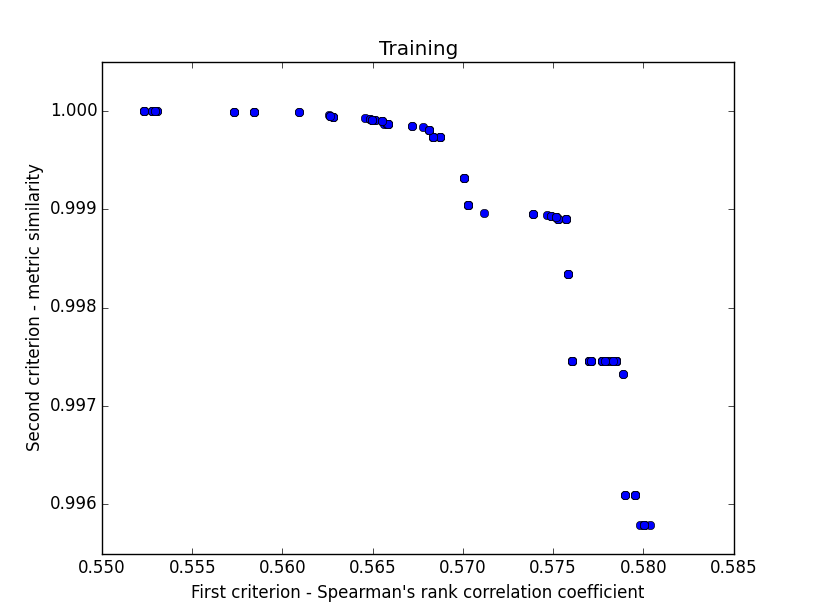
\includegraphics[width=\columnwidth]{Images/nsgaTraining.PNG}
	\centering
	\caption{Results of the first Pareto front of the second run on the training set.}	
	\label{fig:NSGABestTraining}
\end{figure}

\begin{figure}	
	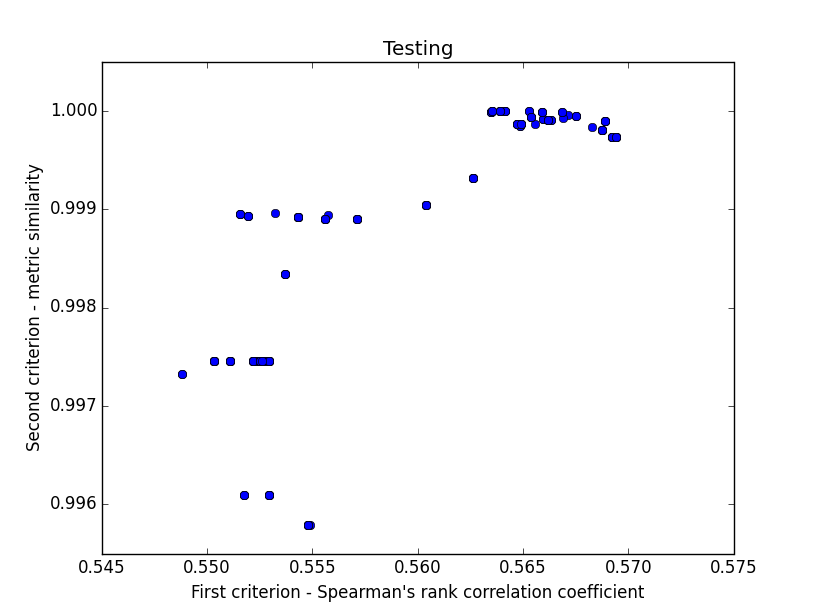
\includegraphics[width=\columnwidth]{Images/nsgaValidation.PNG}
	\centering
	\caption{Results of the first Pareto front of the second run on the testing set. Note the high correlation between both criteria - the higher values of the accuracy criterion are associated with higher values of the metric similarity criterion.}	
	\label{fig:NSGABestValidation}
\end{figure}